\documentclass[msc]{ppgccufmg}    % ou [msc] para disserta��es
                                  % de mestrado. Para propostas ou
                                  % projetos, usar [phd,project],
                                  % [msc,proposal], etc.

%\usepackage[brazil]{babel}        % se o documento for em portugu�s, OU
\usepackage[english]{babel}      % se o documento for em ingl�s
\usepackage[latin1]{inputenc}
\usepackage[T1]{fontenc}
\usepackage{type1ec}
\usepackage{graphicx}
\usepackage[a4paper,
  portuguese,
  bookmarks=true,
  bookmarksnumbered=true,
  linktocpage,
  colorlinks,
  citecolor=black,
  urlcolor=black,
  linkcolor=black,
  filecolor=black,
  ]{hyperref}
\usepackage[square]{natbib}

%%%%%%%%%%%%%%%%%%%%%%%%%%%%%%%%%%%%%%%%
\usepackage{hyperref}
\usepackage{paralist}
%\usepackage{graphicx}
\usepackage{tikz}
\usepackage{xcolor,xspace}
\usepackage{thmtools}
\usepackage{amsmath,amssymb}
\usepackage{mathpartir}
\usepackage{lettrine}
\usepackage[modulo]{lineno}
\usepackage{lipsum}

\usepackage{afterpage}


\declaretheorem[style=definition]{example}
\declaretheorem[style=proof]{proof}
\declaretheorem[style=definition]{definition}
\declaretheorem[style=definition]{proposition}

\newcommand{\auxFun}[1]{\mbox{\textbf{#1}}}
\newcommand\loc[1]{\mbox{\textsf{loc}$_{#1}$}}
\newcommand\gr{\xspace\mbox{GR}\xspace}
\newcommand\lr{\xspace\mbox{LR}\xspace}
\newcommand{\cupdot}{\mathbin{\mathaccent\cdot\cup}}
\newcommand\supp{\xspace\mbox{supp}\xspace}
\newcommand{\lb}[1]{\mbox{$#1$}_{\downarrow}}
\newcommand{\ub}[1]{\mbox{$#1$}_{\uparrow}}

\newcommand{\code}[1]{\mbox{#1}}
\newcommand\ranboxes{\mbox{\textsf{SymbRanges}~}}
\newcommand\memboxes{\mbox{\textsf{MemLocs}~}}
\newcommand\mytrue{\mbox{\textsf{True}~}}
\newcommand\myfalse{\mbox{\textsf{False}~}}
%%%%%%%%%%%%%%%%%%%%%%%%%%%%%%%%%%%%%%%%

\begin{document}

% O comando a seguir, \ppgccufmg, prov� todas as informa��es relevantes para a
% classe ppgccufmg. Por favor, consulte a documenta��o para a descri��o de
% cada chave.

% Um exemplo para documentos em portugu�s � apresentado a seguir:
\ppgccufmg{
  title={Symbolic Range Analysis of Pointers},
  portuguesetitle={An�lise Simb�lica de Intervalos de Ponteiros},
  authorrev={Mendes Paisante, Vitor},
  cutter={???},
  cdu={???},
  university={Federal University of Minas Gerais},
  portugueseuniversity={Universidade Federal de Minas Gerais},
  course={Computer Science},
  portuguesecourse={Ci�ncia da Computa��o},
  address={Belo Horizonte},
  date={2016-07},
  keywords={Alias Analysis, Static Analysis, Compilers},
  advisor={Fernando Magno Quint�o Pereira},
  coadvisor={Leonardo Barbosa e Oliveria},
%  approval={img/approvalsheet.eps},
%  approval=[-2.5cm][1]{aprovalsheet},
  abstract={Resumo}{resumo},
  abstract=[english]{Abstract}{abstract},
%  abstract={Extended Abstract}{resumoest},
  dedication={dedicatoria},
  ack={agradecimentos},
%  ack=[Acknowledgments]{ack},
  epigraphtext={'Are we nearly there?' Alice managed to
pant out at last.\\ 'Nearly there!' the Queen repeated. 'Why, we
passed it ten minutes ago! Faster!'}{Lewis Carroll},
  indexkeys={1.~Computa��o. 2.~Compiladores. 3.~An�lise Est�tica I.~Orientador.
    II.~T�tulo.},
}

% Um exemplo para documentos em ingl�s � apresentado a seguir (lembre-se de
% usar \usepackage[english]{babel}):
%\ppgccufmg{
%  title={Protocol for Error-Verification inside\\Totally Error-Free
%    Networks},
%  authorrev={da Camara Neto, Vilar Fiuza},
%  cutter={D1234p},
%  cdu={519.6*82.10},
%  university={Federal University of Minas Gerais},
%  course={Computer Science},
%  portuguesetitle={Protocolo para Verifica��o de Erros\\em Redes Totalmente
%    Confi�veis},
%  portugueseuniversity={Universidade Federal de Minas Gerais},
%  portuguesecourse={Ci�ncia da Computa��o},
%  address={Belo Horizonte},
%  date={2008-03},
%  advisor={Adamastor Pompeu Set�bal},
%  approval={img/approvalsheet.eps},
%  abstract=[brazil]{Resumo}{resumo},
%  abstract={Abstract}{abstract},
%  dedication={dedicatoria},
%  ack={agradecimentos},
%  epigraphtext={Truth and lie are opposite things.}{Unknown},
%}

%Chapter 1: Introduction
\chapter{Introduction}
\label {chap:introduction}
\section {Context}
% the importance of Alias Analysis
Pointer analysis is one of the most fundamental compiler technologies.
This analysis lets the compiler distinguish one memory location from others;
hence, it provides the necessary information to transform code that manipulates
memory.
Given this importance, it comes as no surprise that pointer analysis has been
one of the most researched topics within the field of compiler
construction~\citep{Hind01}.
This research has contributed to make the present algorithms more
precise~\citep{Hardekopf07a,Zhang14}, and faster~\citep{Hardekopf11,Shang12}.
Nevertheless, one particular feature of imperative programming languages remains
to be handled satisfactorily by the current state-of-the-art approaches:
the disambiguation of pointer intervals.

\section {Problem}
% The problem imposed by pointer arithmetics and The need for better alias analyses.
Mainstream compilers still struggle to distinguish intervals within the
same array.
In other words, state-of-the-art pointer analyses often fail to disambiguate
regions addressed from a common base pointer via different
offsets, as explained by Yong and Horwitz~\citep{Yong04}. Figure 
\ref{fig:intro_ex} shows an example that state-of-the-art pointer analyses 
tend not to deal with satisfactorily. In the example, both stores on the $r$ 
array posses different offsets and they do not alias. To figure out that such 
offsets are disjoint it is necessary to verify their ranges and add a new layer
of analysis to the current pointer analyses available.

\begin{figure}[t!]
  \centering
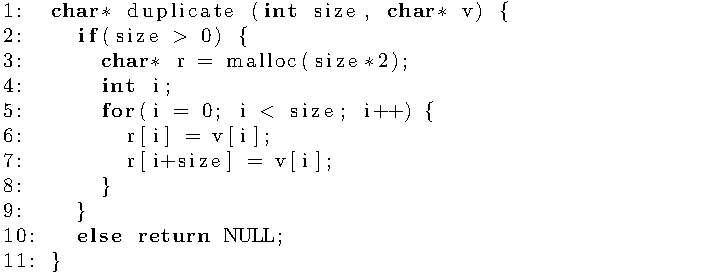
\includegraphics[width=\linewidth]{img/introex}
  \caption{Example.}
  \label{fig:intro_ex}
\end{figure}

Field-sensitive pointer analysis, provide a partial solution to this problem.
These analyses can distinguish different fields within a record, such
as a struct in C~\citep{Pearce04}, or a class in Java~\citep{Yan11}.
However, they rely on syntax that is usually absent in the low level program
representations adopted by compilers.
Shape analyses~\citep{Jones82,Sagiv98} can disambiguate subparts of
data-structures such as arrays, yet their scalability remains an issue to be
solved.
Consequently, many compiler optimizations, such as
loop transformations, tiling, fission, skewing and
interchanging~\citep[Ch.09]{Wolfe96}, are very limited in practice.
Therefore, we claim that, to reach their full potential, compilers need to
be provided with more effective alias analyses.

\section {Solution}
% Combining alias and range analyses.
This work describes such an analysis.
We introduce an abstract domain that associates pointers with symbolic ranges.
In other words, for each pointer $p$ we conservatively estimate the range of
memory slots that can be addressed as an offset of $p$.
We let $\gr(p)$ be the global abstract address set associated with pointer $p$, 
such that if
$\loc{i} + [l, u] \in \gr(p)$, then $p$ may dereference any address
from $@(\loc{i}) + l$ to $@(\loc{i}) + u$,
where $\loc{i}$ is a program site that
contains a memory allocation call, and $@(\loc{i})$ is the actual return
address of the {\em malloc} at runtime.
We let $\{ l, u \}$ be two {\em symbols} defined within the program code.
Like the vast majority of pointer analyses available in the compiler
literature, from Andersen's work~\citep{Andersen94} to the more recent 
technique of Zhang {\em et al.}~\citep{Zhang14}, our method is correct if the
underlying program is also correct.
In other words, our results are sound with respect to the semantics of the
program if this program has no undefined behavior, such as out-of-bounds
accesses.

\textbf{The key insight of our research} is the combination of pointer analysis
with range analysis on the symbolic interval lattice.
In a symbolic range analysis, ranges are defined as expressions of the program's
symbols, a symbol being either a constant or the name of a variable.
There exist many approaches to symbolic range analyses in the
literature~\citep{Blume94,Nazare14,Rugina05}.
The algorithms that we present in this work do not depend on any particular
implementation.
Nevertheless, the more precise the range analysis that we use, the more
precise the analysis facts that we produce.
In this work we have adopted the symbolic range analysis proposed in 1994 by
William Blume and Rudolf Eigenmann~\citep{Blume94}.

\section {Summary of experimental results}
To validate our ideas, we have implemented them in the LLVM compilation
infra-structure~\citep{Lattner04}.
We have tested our pointer analysis onto three different benchmarks
used in previous work related to pointer disambiguation:
Prolangs~\citep{Ryder01}, PtrDist~\citep{Zhao05} and MallocBench~\citep{Grunwald93}.
As we show in Chapter \ref{chap:exp}, our analysis is linear on the size of
programs.
It can go over one-million assembly instructions in approximately 10 seconds.
Furthermore, we can disambiguate 1.35x more queries than the alias analysis
currently available in LLVM.

\section {Summary of publications}
The analysis described here was published on the International Symposium on 
Code Generation and Optimization (CGO) of 2016 held in Barcelona, Spain 
\citep{Paisante16}. 

The technology behind it is also present on two other publications 
\citep{Paisante14, Saggioro15}. In them, we've used the algorithm presented here
to infer the layout and the content of buffers transfered through the network. 
This was useful for verifying, in a safe communication line, if the information 
transfered between two programs through a network should be considered potentially 
dangerous or not. If proven not dangerous, guards for checking integer overflows
may not be necessary. These articles proposed methods for such verification to 
be used on the internet of things (IoT), where simple devices could run 
significantly faster with a reduced number of integer overflow checks. 
The layout and content inference analysis used in these papers differed to our 
current approach by using a numerical range analysis, since a symbolic approach 
would not be of relevance for such application.

\section {Next Chapters}

This work is divided in the following structure: 
\begin{itemize}
\item Chapter \ref{chap:introduction} presented an introduction describing the context
of points-to analysis, the problem faced by this work, our solution of adding 
a layer of symbolic range analysis to points-to analysis, and our publications.
\item Chapter \ref{chap:background} presents the background behind our work, the 
concepts and other works used. It also does a literature review of other related 
publications. The topics and concepts it covers are the SSA form, the LLVM 
compiler framework, points-to analysis, range analysis, the use of pointer 
disambiguation for automatic parallelization of code and the merging of 
points-to analysis with range analysis. 
\item Chapter \ref{chap:work} describes our points-to analysis. It gives an 
overview of our algorithm, shows how we combine the symbolic range analysis 
with pointer analysis, describes the local and global parts of our work, 
discusses about the algorithm's complexity and end with an example. 
\item Chapter \ref{chap:exp} shows our experiments and results. 
\item Chapter \ref{chap:final} concludes this dissertation. It shows the
limitations of our work, discusses future work to be done and issues final
conclusions.
\end{itemize}

%Chapter 2: Literature Review
\chapter{Background}
\label {chap:background}

%\section {Background}
%This section elaborates on a few key concepts and technologies used in this 
%work. Later sections give a more in depth look into the main concepts associated 
%with our approach.
\section {SSA form} %\subsection {SSA form}
Data structure choices directly influence in the power and efficiency of program
optimizations in our current optimizing compilers. Choosing poorly which data
structures to use can inhibit program optimization to a point where  advanced 
techniques can become undesirable. The static single assignment form (SSA) makes
a useful class of optimizations more efficient and powerful. It was initially
proposed in the 80s to, among other uses, verify the equality of variables in a 
program \citep{Alpern88}.

Consider the program slice in figure \ref{fig:ssa_ex}. Could it be said that $I$ 
and $J$ are equivalent? Such answer will depend on which program point the 
execution is currently. In the end of the \textbf{if-then-else} the answer will 
depend, dynamically, on the value of $Q$, or no answer can be defined in a
conservative static approach. However, in program point $4$, these variables 
are equal even on the static view. To allow the detection of such equivalences 
without taking into account different points in the program, it's necessary 
to add several new variables for each variable in the original program. So, 
in the example, it is necessary to break $I$ into three distinct variables. One
in the \textbf{then} clause, one in the \textbf{else} clause and a last one in 
the end of the \textbf{if-then-else}. The same is done for $J$ and now it's 
possible to verify, statically, that the $I$ and $J$ from inside the 
\textbf{then} clause are equivalent. 

\begin{figure}[t!]
  \centering
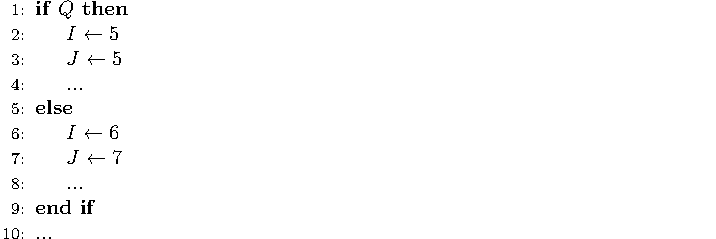
\includegraphics[width=\linewidth]{img/ssa_ex}
  \caption{Example where the SSA form can improve on the value numbering
   optimization.}
  \label{fig:ssa_ex}
\end{figure}

%first step
The process of transforming a program into the SSA form requires two steps 
\citep{Cytron89}.
The first step consists in inserting $\phi$-functions into certain points on the 
program. Such functions are special assignment states in the form $U\gets\phi
(V,W,...)$, where $U,V,W,...$ are variables and the number of  operands 
$V,W,...$ is the number of control flow predecessors of the program point where
the $\phi$-function is inserted. Such control flow predecessors are listed in 
order where the $j$th operand is associated with the $j$th predecessor. If 
the program execution reaches the $\phi$-function from its $j$th predecessor, 
then $U$ is assigned the value of the $j$th operand. Each execution of a $\phi$ 
statement uses only one operand and which operand to be used depends on the 
flow of execution. A $\phi$-function can be trivially placed for each variable 
$V$ int the form $V\gets\phi(V,V,...)$ at the entrance to any CFG node in the 
program without changing semantics.

%second step
The second step consists in giving new names for each variable V in the form 
$V_i$ for various integers i. Each mention of $V$ in the program is replaced 
by a mention of ones of these new names of $V$. Each new name $V_i$ for $V$ is
the target of exactly one assignment statement in the program text. And along 
any control flow path, if you consider any use of a new name $V_i$ for $V$ and 
the corresponding use of $V$ in the original program, $V$ and $V_i$ will have 
the same value. 

%minimal SSA
A program is in $minimalSSA$ form if it is in SSA form and if the number of 
$\phi$-functions inserted is as small as possible \citep{Rosen88}. Extra 
$\phi$-functions (more than the $minimalSSA$ form) might inhibit optimizations 
by hiding useful facts. They also add unnecessary overhead to the process of 
optimization. Thus it is very important to place $\phi$-functions only where 
they are required to maintain the SSA form.

%ssa conclusion
After a program has been transformed into the static single assignment form 
(SSA), it has two useful properties. First, each use of a variable is reached 
by exactly one assignment to that variable. Secondly, the programs contains 
$\phi$-functions that distinguish values of variables obtained through distinct
incoming control flow paths.

%e-ssa
The Extended Static Single Assignment form is a cheaply computable extension of
SSA \citep{Bodik00}. This extension differs from the $minimalSSA$ form by 
introducing $\sigma$-functions that redefine the program's variables in 
points of interest, such as branches and switches. The main advantage of this 
$\sigma$-functions are inserted, for each variable appearing in the conditional 
expression, into the CFP out-edges of the conditional branch. Because of these
assignments, each outcome of the conditional is associated with a distinct 
variable name, which allows for splitting the ranges of the conditional 
variables in range analysis, for example, with each of its $\sigma$-assignments
taking distinct pieces of their range. The $\sigma$-functions are usually placed 
at the beginning of the basic blocks targeted by the branch.

\begin{figure}[t!]
  \centering
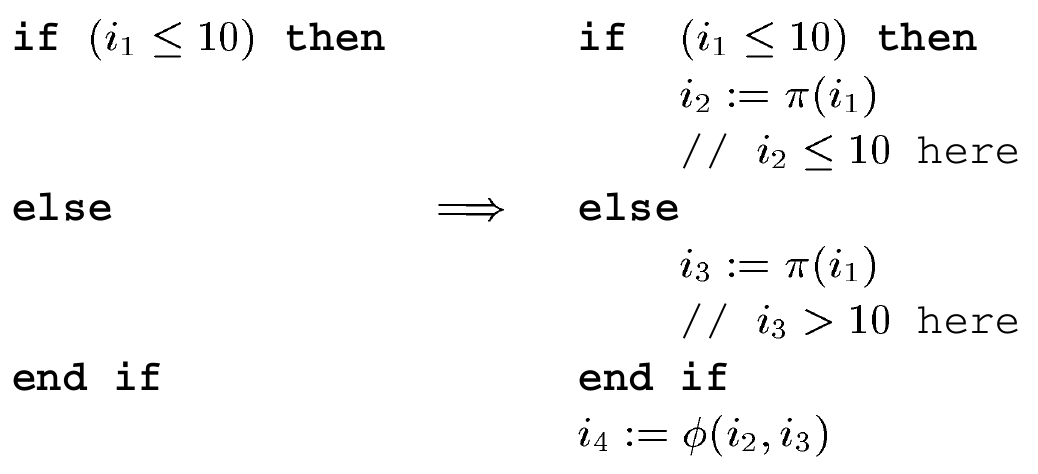
\includegraphics[width=300px]{img/essa}
  \caption{Example showing the Extended Static Single Assignment form 
  transformation by inserting $\sigma$-functions.}
  \label{fig:essa}
\end{figure}

%\subsection {Control Flow Graphs}

\section{LLVM} %\subsection {LLVM}
LLVM (Low-Level Virtual Machine) \citep{Lattner04} 
is a compiler framework that aims to make
program analyses and transformations available for any piece of software in a 
transparent way for the programmers. It has two main characteristics are a code
representation with several features that serve as common a representation 
for analyses and transformations and machine code translation, and a compiler 
design that exploits its representation to provide a multitude of capabilities.

The LLVM code representation uses a RISC-like instruction set allied to 
higher level information to describe programs in a useful way for analyses and 
transformations. This higher level information includes type information, 
explicit control flow graphs and an explicit data-flow representation using an
infinite, typed register set in the SSA form. This code representation has 
several features, such as a low-level language independent type system that can 
be used to implement data-types and operations from higher-level languages, 
instructions for performing type conversions and address arithmetic, and two
low-level exceptions-handling instructions for implementing exception semantics 
from languages who have it. The LLVM representation is independent from the 
source code language and it utilizes a low-level instruction set and memory 
model that are only slightly richer than common assembly languages. Its type 
system does not prevent representing code with very little type information and 
it does not impose any particular runtime requirement on programs.

The LLVM compiler framework exploits its code representation to provide a 
combination of five capabilities: persistent program information, offline code 
generation, user-based profiling and optimization, transparent runtime model and
uniform, whole-program compilation. Over the last ten years, LLVM has 
somewhat altered this landscape and it is now used as a common 
infrastructure to implement a broad variety of statically and runtime compiled 
languages. We've used it to implement the analysis present in this work.

%\subsection {Lattice}

\section {Points-to Analysis}
%- Work on points-to analysis
The contribution of this work is a new representation of pointers, based
on the \ranboxes lattice, and an algorithm to reach a fixed point in this
lattice, based on abstract interpretation.
This contribution complements classic work on pointer analysis.
In other words, our representation of pointers can be used to enhance the
precision of algorithms such as
Steensgard's~\citep{Steensgaard96}, Andersen's~\citep{Andersen94}, or even
the state-of-the-art technique of Hardekopf and Lin~\citep{Hardekopf11}.
These techniques map pointers to sets of locations, but they could be
augmented to map pointers to sets of locations plus ranges.
Furthermore, the use of our approach does not prevent the employment of
acceleration techniques such as lazy cycle detection~\citep{Hardekopf07a}, or
wave propagation~\citep{Pereira09b}.

Another analysis technique, originally investigated by Reynolds 
~\citep{Reynolds68} for a Lisp-like language, is shape-analysis and it aims to 
give, for each program point a finite characterization of the possible 
"shapes" that the program's heap-allocated data structures can have at that 
point. Shapes characterize data structures. 
A shape descriptor could indicate whether the heap contains a singly linked 
list, potentially with a cycle, a doubly linked list, a binary tree, and so on.
Shape Analysis is a static code analysis 
that discovers and verifies properties of linked, dynamically 
allocated data structures in computer programs. It is a form of 
pointer analysis, although it is more precise than typical pointer analysis.
It has been applied to a variety of problems, such as memory safety and finding 
memory leaks, dereferences of dangling pointers, and 
discovering cases where a block of memory is freed more than once,
finding array out-of-bounds errors, checking type-state properties, and 
verifying that a sort method is correct.

\section {Range Analysis}
%- Work on range analysis
Range Analysis is a compiler technique that aims to to find, statically, minimum
and maximum values that each program variable might assume during the program 
execution. This analysis is important for enabling several compiler 
optimizations, such as dead and redundant code elimination. These are the 
removal of array bounds checks \citep{Logozzo08} and overflow \citep{Sol11} 
checks for example. It can also be used for bitwidth aware register allocation
\citep{Barik06}, branch prediction \citep{Patterson95} and synthesis of hardware
for specific applications \citep{Cong05}.

The approach of simply having integer values as minimums and maximums may enable
several compiler optimizations, but it is not effective do validate memory 
accesses or handle pointers. We adopt in this work a symbolic range analysis 
\citep{Nazare14}. The analysis we use adopts symbolic ranges and a symbolic
kernel, which is a set formed by either constants known statically or variables 
defined as input values, such as formal parameters of functions, reads and 
loads. An abstract interpretation framework generates invariants as symbolic 
ranges over the program's symbolic kernel, extracts a set of interval 
constraints from the program and performs a fix-point algorithm until 
convergence. 

The symbolic range analysis uses symbolic expressions for the lower and upper 
bounds of ranges. $E$ is a symbolic expression, if and only if, $E$ is defined 
by the grammar below. In this grammar $s$ is a symbol and $n \in \mathbb{N}$. 
 
{\centering $E~::=~n~|~s~|~min(E,E)~|~max(E,E)~|~E-E~|~E+E~|~E/E~|~E mod E~|~E*E$}

Even though there is a natural lattice between integer values coupled with both
positive and negative infinities, there is no ordering between two distinct
elements of the symbolic kernel of a program. The analysis provides a way to 
define such ordering with a valuation of symbolic expressions.

\section {Pointer Disambiguation for Parallelization}
%- Work on pointer disambiguation for parallelization
There exist previous work that used similar lattices as ours, albeit different
resolution algorithms.
For instance, much of the work on automatic parallelization has some way to
associate symbolic offsets, usually loop bounds, with pointers.
Michael Wolfe~\citep[Ch.7]{Wolfe96} and Aho {et al.}~\citep[Ch.11]{Aho06} have 
entire chapters devoted to this issue.
The key difference between our work and this line of research is the algorithm
to solve pointer relations: they resort to integer linear programming (ILP) or
the Greatest Common Divisor test to solve diophantine equations, whereas we
do abstract interpretation.

We believe that the state-of-the-art approach in the field today is Rugina and 
Rinard~\citep{Rugina05}. Their paper presents a novel framework for the symbolic
bounds analysis of pointers, array indexes, and accessed memory regions. 
Instead of using traditional fixed-point algorithms, it formulates each analysis 
problem as a system of inequality constraints between symbolic bound 
polynomials. It then reduces the constraint system to a linear program. The 
solution to the linear program provides symbolic lower and upper bounds for 
the values of pointer and array index variables and for the regions of memory 
that each statement and procedure accesses.
Their technique was applied to divide and conquer programs that access disjoint 
regions of dynamically allocated arrays. Experimental results showed that their 
algorithm can verify the absence of data races in benchmark parallel programs, 
detect the available parallelism in benchmark serial programs, and verify that 
both sets of benchmark programs do not violate their array bounds.

We speculate that the ILP approach is too expensive to be used in large 
programs; hence, concessions must be made for the sake of speed.
For instance, whereas the previous literature that we know restrict their
work to pointers within loops, we can analyze programs with over one million
assembly instructions in a few seconds.
\section {Points-to with Range Analyses}
%- Previous attempts to merge points-to and range analyses
There exist work that, like ours, also associates intervals with pointers, and
solves static analysis via abstract interpretation techniques.
However, to the best of our knowledge, these approaches have a fundamental
difference to our work: they use integer intervals a l\`{a}
Cousot~\citep{Cousot77}, whereas we use symbolic intervals.
The inspiration for much of this work springs from Balakrishnan and Reps notion
of {\em Value Set} Analysis~\citep{Balakrishnan04}.
Integer intervals have also being used by Yong {\em et al.}~\citep{Yong04} and,
more recently, by Oh {\em et al.}~\citep{Oh14}.
In the latter case, Oh {\em et al.} use pointer disambiguation incidentally, to
demonstrate their ability to implement efficiently static analyses in a
context-sensitive way.
Even though integer ranges fit well the need of machine code, as demonstrated
by Balakrishnan and Reps, we believe that further precision requires more
expressive lattices.
We have not implemented value set analysis, but we have tried a simple
experiment: we counted the number of pointers that have integer ranges, and
compared this number against the quantity of pointers that have symbolic ranges.
We found out that 20.47\% of the pointers in our three benchmark suites have
exclusively symbolic ranges.
Classic range analysis would not be able to distinguish them.
Notice that numeric ranges are more common among pointer variables than among
integer, because fields within {\em structs} -- a very common construct in C -- are
indexed through integers.
Finally, the fact that we use Bodik's e-SSA form~\citep{Bodik00} distinguish our
abstract interpretation algorithm from previous work.
This representation lets us solve our analysis sparsely, whereas Balakrishnan's
algorithm works on a dense representation that associates facts with
pairs formed by variables and program points.

%Chapter 3: A New Points-to Analysis
\chapter{A New Points-to Analysis}
\label {chap:work}

\section{Overview}
\label{sec:ovf}

We have two different ways to answer the
following question: ``do pointers $\mathit{tmp}_i$ and $\mathit{tmp}_j$
alias?"
These tests are called {\em global} and {\em local}.
In this section, we will use two different examples to illustrate situations
in which each query is more effective.
These distinct strategies are complementary: one is not a superset of the other.

\noindent
\textbf{Global pointer disambiguation. }
Figure~\ref{fig:exmotiv} illustrates our first approach to disambiguate
pointers.
The figure shows a pattern typically found in distributed systems
implemented in C.
Messages are represented as arrays of bytes.
In this particular example, messages have two parts: an identifier, which is stored in the beginning of the array, and a payload, which is stored right
after.
The loops in lines 5-8 and 9-12 fill up each of these parts with data.
If a compiler can prove that the stores at lines 6 and 10 are always
independent, then it can perform optimizations that would not be
possible otherwise.
For instance, it can parallelize the loops, or switch them, or merge them into a
single body.

\begin{figure}[t!]
  \centering
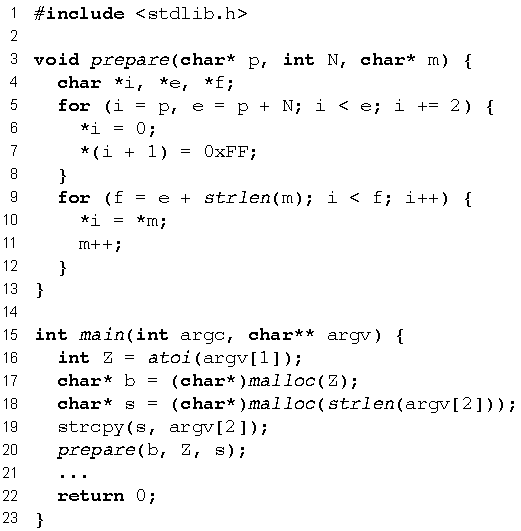
\includegraphics{img/ex0_src.pdf}
  \caption{Example of program that builds up messages as sequences of
  serialized bytes. We are interested in disambiguating the locations accessed
  at lines 6 and 10.}
  \label{fig:exmotiv}
\end{figure}

No alias analysis currently available in either gcc or LLVM is able to
disambiguate the stores at lines 6 and 10.
These analyses are limited because they do not contain {\em range information}.
The range interval $[l, u]$ associated with a variable $i$ is
an estimate of
the lowest ($l$) and highest ($u$) values that $i$ can assume
throughout the execution of the program.
In this work, we propose an alias analysis that solves this problem.
To achieve this goal, we couple this alias analysis with range
analysis on symbolic intervals~\citep{Blume94}.
Thus, we will say that the store at line 6 might modify any address from
$\mathtt{p} + 0$ to $\mathtt{p} + \mathtt{N} - 1$, and that the store at line 10
might write on any address from $\mathtt{p} + N$ to $\mathtt{p} + N + 
\mathtt{strlen(m) - 1}$.
For this purpose, we will use an \emph{abstract address} that
encodes the actual value(s) of $p$ inside the $\mathtt{prepare}$
function.
These memory addresses are depicted in Figure \ref{fig:pointer_range}, where each
$\square$ represents a memory slot.

\begin{figure}[t!]
\begin{small}
  \centering
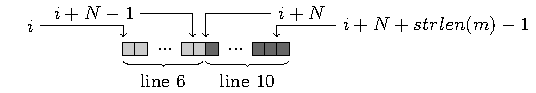
\includegraphics{img/pointer_range_Maroua}
  \caption{Array $p$ in the routine \texttt{prepare} seen in
    Fig.\ref{fig:exmotiv}. Lines 6 and 10 represent the different stores in the figure.}
  \label{fig:pointer_range}
\end{small}
\end{figure}

% How to disambiguate queries:
Whole program analysis reveals that there are two candidate locations
that any pointer in the program may refer to.
These locations have been created at lines 17 and 18 of Figure~\ref{fig:exmotiv},
and we represent them abstractly as $\loc{17}$ and  $\loc{18}$.
These names are unique across the entire program.
After running our analysis, we find out that the abstract state ($\gr$) of
\texttt{i} at line 6 is
$\gr(\mathtt{i}_{\ell{}n.6}) = \{ \loc{17} + [0, \mathtt{N} - 1]$,
and that the abstract state of \texttt{i} at line 10 is
$\gr(\mathtt{i}_{\ell{}n.10}) = \{ \loc{17} + [\mathtt{N}, \mathtt{N + strlen}(m) - 1]
\}$.
Given that these two abstract ranges do not intersect, we know that
the two stores update always different locations.
We call this check the {\em global disambiguation
  criterion}.

\begin{figure}[t!]
  \centering
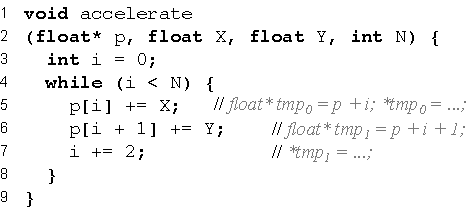
\includegraphics{img/ex4_src}
  \caption{Program that shows the need to assign common names to addresses that spring from the same base pointer.}
  \label{fig:ex4_src}
\end{figure}

\begin{figure}[t!]
  \centering
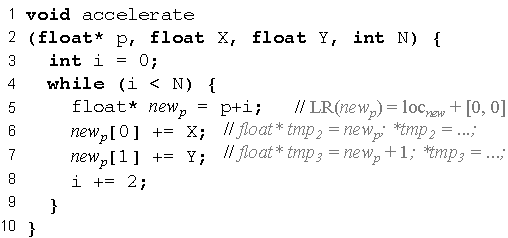
\includegraphics{img/ex4_norm}
  \caption{Program from Figure~\ref{fig:ex4_src}, after pointer is renamed
  within loop.}
  \label{fig:ex4_norm}
\end{figure}

\textbf{Local pointer disambiguation. } Figure~\ref{fig:ex4_src} shows
a program in which the simple intersection of ranges would not let us
disambiguate pointers $\mathit{tmp}_0$ and $\mathit{tmp}_1$.  After
solving global range analysis for that program, we have that
$\gr(\mathit{tmp}_0) = \{ \loc{0} + [0, N + 1] \}$ and that
$\gr(\mathit{tmp}_1) = \{ \loc{0} + [1, N + 2] \}$, where $\loc{0}$
defines the abstract address of the function parameter $p$.  The
intersection of these ranges is non-empty for $N \geq 1$.  Thus, the
global check that we have used to disambiguate locations in
Figure~\ref{fig:exmotiv} does not work in Figure~\ref{fig:ex4_src}.
Notwithstanding this fact, we know that $\mathit{tmp}_0$ and
$\mathit{tmp}_1$ will never point to a common location.  In fact,
these pointers constitute different offsets from the same base
address.
To deal with this imprecision of the global check, we will be also discussing
a {\em local disambiguation criterion}.
In this case, we rename every pointer $p$ that is alive at the beginning of
a single entry region to a fresh name $new_{p}$.
Whereas we use the global test for pointers in different regions, the
local test is applied onto pointers within the same single entry region.
After renaming, we update the table of pointer pairs, so that
$\lr(new_p) = \loc{new} + [0, 0]$, regardless of the old ranges assigned to
the original pointer $p$.
In Figure~\ref{fig:ex4_norm} we would have that
$\lr(\mathit{tmp}_2) =  \loc{new} + [0, 0]$  and
$\lr(\mathit{tmp}_3) =  \loc{new} + [1, 1]$, where $\mathit{tmp_2}$ is
the name of the address $\mathit{new}_p[0]$, and
$\mathit{tmp_3}$ is the name of the address $\mathit{new}_p[1]$.
This new binding of intervals to pointers gives us empty
intersections between similar locations in $\lr(tmp_2)$ and $\lr(tmp_3)$.
Consequently, the local check is able to distinguish addresses referenced by
$\mathit{tmp}_2$ and $\mathit{tmp}_3$.

\section{Combining Range and Pointer Analyses}
\label{sec:sol}

We perform our pointer analysis in several steps.
Figure~\ref{fig:infrastructure} shows how each of these phases relates to each
other.
Our final product is a function 
that, given two pointers, $p_0$ and $p_1$,
tells if they may point to overlapping areas or not.
An invocation of this function is called a {\em query}.
We use an off-the-shelf symbolic range analysis, e.g., \`{a} la
Blume~\citep{Blume94}, to bootstrap our pointer analysis.
By inferring the symbolic ranges of pointers, we have two alias tests: the global
and the local approach.
In the rest of this section we describe each one of these contributions.

\begin{figure}[t!]
  \centering
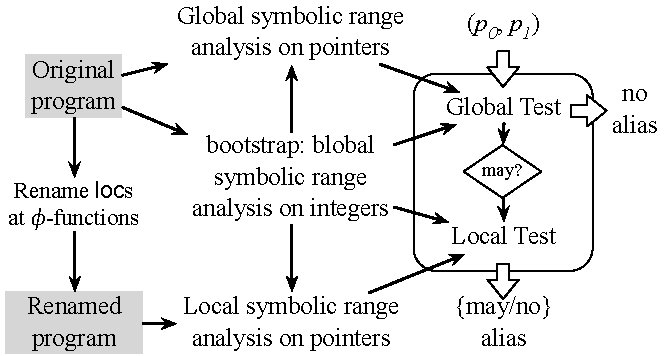
\includegraphics{img/infrastructure}
  \caption{Overview of our pointer analysis.}
  \label{fig:infrastructure}
\end{figure}

\subsection{A Core Language}
\label{sub:lang}

We solve range analysis through abstract interpretation.
To explain how we abstract each instruction in our intermediate representation,
we shall use the language seen in Figure~\ref{fig:syntax};
henceforth, we shall call this syntax our {\em core language}.
We shall be working on programs in Extended Static Single Assignment (e-SSA)
form~\citep{Bodik00}.
E-SSA form is a flavor of Static Single Assignment (SSA)~\citep{Cytron91} form,
with variable renaming after inequalities.
Thus, our core language contains $\phi$-functions to ensure the single
definition (SSA) property, and intersections to rename variables after
conditionals.
We assume that $\phi$-functions have only two arguments.
Generalizing this notation to $n$-ary functions is immediate.

\begin{table}[t!]
\begin{footnotesize}
\renewcommand\arraystretch{1}
\begin{center}
\begin{tabular}{lcl}
Integer constants               & ::= & $\{c_1, c_2, \ldots\}$ \\
Integer variables               & ::= & $\{i_1, i_2, \ldots\}$ \\
Pointer variables               & ::= & $\{p_1, p_2, \ldots\}$ \\
Instructions (I)                & ::= & \\
-- Allocate memory              & $|$ & $p_0 = \code{malloc}(i_0)$ \\
-- Free memory                  & $|$ & $p_0 = \code{free}(p_1)$ \\
-- Pointer plus int             & $|$ & $p_0 = p_1 + i_0$ \\
-- Pointer plus const           & $|$ & $p_0 = p_1 + c_0$ \\
-- Bound intersection           & $|$ & $p_0 = p_1 \cap [l, u]$ \\
-- Load into pointer            & $|$ & $p_0 = *p_1$ \\
-- Store from pointer           & $|$ & $*p_0 = p_1$ \\
-- $\phi$-function              & $|$ & $p_0 =\phi(p_1:\ell_1, p_2:\ell_2)$ \\
-- Branch if not zero           & $|$ & $\code{bnz}(v, \ell)$ \\
-- Unconditional jump           & $|$ & $\code{jump}(\ell)$ \\
\end{tabular}
\end{center}
\caption{The syntax of our language of pointers.}
\label{fig:syntax}
\end{footnotesize}
\end{table}

Figure~\ref{fig:ex3} shows the control flow graph of the program seen in
Figure~\ref{fig:exmotiv}.
The implementation of the analysis that we shall present in this work is
interprocedural, albeit
not context-sensitive.
To achieve interprocedurality, we associate actual parameters with formal parameters 
of functions.
In the example of Figure~\ref{fig:exmotiv}, pointer $b$ -- an actual parameter --
is linked with
$p$ -- a formal parameter -- through a $\phi$-function.

\begin{figure}[t!]
  \centering
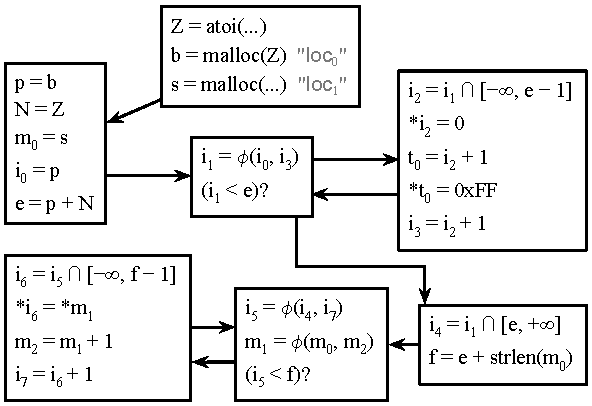
\includegraphics{img/ex3}
  \caption{Control flow graph of program seen in Figure~\ref{fig:exmotiv}}
  \label{fig:ex3}
\end{figure}

The e-SSA format lets us implement our analysis sparsely, e.g,. we can assign
information directly to variables, instead of pairs of variables and program
points.
As demonstrated by Choi {\em et al.}~\citep{Choi91}, the main advantage of a sparse
analysis is efficiency: the product of the analysis - the information that is
bound to each variable - requires $O(N)$ space, where $N$ is the number of
variable names in the program.
Furthermore, as we shall explain in the rest of this section, our analysis
can be computed in $O(N)$ time.

Key to these good properties is the fact that we create new variable names
at each program point where our analysis can infer new information.
This knowledge appears due to memory allocation (malloc), deallocation
(free), pointer arithmetic, intersections and $\phi$-functions.
Each of these instructions defines new variables, whose names are associated
with information.
For instance, the instruction $p_0 = \code{free}(p_1)$ copies $p_1$ to $p_0$,
and binds $p_0$ to a memory chunk of size 0.
As we will show in Section~\ref{sub:global}, our abstract interpreter associates
with $p_0$ a new abstract state which indicates that $p_0$ is not a valid
reference to any location.

\subsection{Program Locations.}
\label{sub:loc}

Our analysis binds variable names to sets of {\em locations} and {\em ranges}.
We denote the set of locations in a program by
${\mathcal L}oc=\{\loc{0},\loc{1}\ldots, \loc{n-1}\}$ where n is the number of allocation sites.
In our representation, i.e., Figure~\ref{fig:syntax}, new locations are created by
{\em malloc} operations.

\begin{example}[label=initialization]
\label{ex:initialization}
Figure~\ref{fig:ex3} shows the control flow graph of the program  seen
in Figure~\ref{fig:exmotiv}. The two allocations at lines 17 and 18 are
associated respectively with $\loc{0}$ and $\loc{1}$. 
\end{example}

\subsection{Symbolic Range Analysis.}
\label{sub:sra}

We start our pointer analysis by running an off-the-shelf {\em range analysis}
parameterized on {\em symbols}.
For the sake of completeness, we shall revisit the main notions associated with
range analysis, which we borrow from Nazar\'{e} {\em et al.}~\citep{Nazare14}.
We say that $E$ is a symbolic {\em expression}, if and only if, $E$ is
defined by the grammar below.
In this definition, $s$ is a symbol and $n \in \mathbb{N}$.
The set of symbols $s$ in a program form its {\em symbolic kernel}.
The symbolic kernel is formed by names that cannot be represented as function
of other names in the program text.
Concretely, this set contains the names of global variables and variables
assigned with values returned from library functions.
\renewcommand{\arraystretch}{0.9}
\[
\begin{array}{rcl}
E & ::= & n \ \ | \ \ s \ \ | \ \  \mbox{min}(E, E) \ \ | \ \ \mbox{max}(E, E) \ \
 | \ \ E - E \\ &  & | \ \ E + E \ \ | \ \ E / E  \ \ |
 \ \ E \ \mbox{mod} \ E  \ \ | \ \ E \times E 
\end{array}
\]
We shall be performing arithmetic operations over the partially ordered
set $S = S_E \cup \{-\infty, +\infty\}$, where
$S_E$ is the set of symbolic expressions.
The partial ordering is given by $-\infty < \ldots < -2 < -1 < 0 < 1 < 2 <
\ldots +\infty$. 
There exists no ordering between two distinct elements of the symbolic
kernel of a program.
For instance, $N<N+1$ but there is no relationship between an
expression containing $N$ and another expression containing $M$.

A {\em symbolic interval} is a pair $R=[l, u]$, where $l$ and $u$ are
symbolic expressions. We denote by $\lb{R}$ the lower bound $l$ and
$\ub{R}$ the upper bound $u$.
We define the partially ordered set of (symbolic) intervals
$S^2 = (S \times S, \sqsubseteq)$, where the ordering operator is
defined as:
\[
[l_0, u_0] \sqsubseteq [l_1, u_1], \ \mbox{if} \ l_1 \leq l_0 \wedge
u_1 \geq u_0
\]

From the previous definitions, we  define the semi-lattice \ranboxes of symbolic
intervals as $(S^2, \sqsubseteq, \sqcup, \emptyset,$ $[-\infty, +\infty])$,
where the join operator ``$\sqcup$" is defined as:
\[
[a_1, a_2] \sqcup [b_1, b_2] = [\mbox{min}(a_1, b_1), \mbox{max}(a_2, b_2)]
\]
Our lattice has a least element $\emptyset$, such that:
\[ \emptyset \sqcup [l, u] = [l, u] \sqcup \emptyset = [l, u]\]
and a greatest element $[-\infty, +\infty]$, such that:
\[[-\infty, +\infty] \sqcup [l, u] = [l, u] \sqcup [-\infty, +\infty] =
[-\infty, +\infty] \]

For sake of clarity, we also define the intersection operator
``$\sqcap$":
\[
[a_1, a_2] \sqcap [b_1, b_2] =
\begin{cases}
\emptyset, \ \ \mbox{if} \ a_2 < b_1 \ \mbox{or} \ b_2 < a_1 \\
[\mbox{max}(a_1, b_1), \mbox{min}(a_2, b_2)], \mbox{otherwise}
\end{cases}
\]
$[-\infty, +\infty]$ is absorbant and $\emptyset$
is neutral for $\sqcap$.


The result of range analysis is a function $R : V \mapsto S^2$, that maps each
integer variable $i$ in a program to an interval $[l, u], l \leq u$, e.g.,
$R(i) = [l, u]$.
The more precise the technique we use to produce this result, the more precise our
results will be.
Nevertheless, the exact implementation of the range analysis is immaterial for
the formalization that follows.
In this work, we are using the following widening operator on \ranboxes:
 \[[l, u]\nabla [l', u'] \ = \
\begin{cases}
[l, u] & \mbox{if} \ l = l' \ \mbox{and} \ u = u' \\
[l, +\infty] & \mbox{if} \ l = l' \ \mbox{and} \ u' > u \\
[-\infty, u] & \mbox{if} \ l' < l \ \mbox{and} \ u' = u \\
[-\infty, +\infty] & \mbox{if} \ l' < l \ \mbox{and} \ u' > u \\
\end{cases}
\]


The only requirement that we impose on the implementation of range analysis is
that it exists over \ranboxes, our lattice of symbolic intervals.\\  We denote by
$(\alpha_{\mbox{\textsf{SymbRanges}}},\gamma_{\mbox{\textsf{SymbRanges}}})$
    the underlying galois connection.

\begin{example}[label=normalization]
\label{ex:normalization1}
A range analysis such as Nazar\'{e} {\em et al.}'s~\citep{Nazare14}, if
applied onto the program seen in Figure~\ref{fig:ex4_src}, will
gives us that $R(i_{\langle line \ 3\rangle}) = [0, 0],
R(i_{\ell{}n.5}) = [0, N - 1]$,
$R(i_{\ell{}n.7}) = [0, N + 1]$.
\end{example}

\subsection{Global Range Analysis of Pointers}
\label{sub:global}
As we have mentioned in Section~\ref{sec:ovf} we use two different
strategies to disambiguate pointers: the global and the local test.
Our global pointer analysis goes over the entire code of the program,
associating variables that have the pointer type with elements of an
abstract domain that we will define soon.
The local analysis, on the other hand, works only for small regions of the
program text.
We shall discuss the local test in Section~\ref{sub:local}.
In this section, we focus on the global test, which is an
abstract-interpretation based algorithm.

\paragraph{An Abstract Domain of Pointer Locations.}

We associate pointers with tuples of size $n$: $(\ranboxes \cupdot \bot)^n$;
$n$ being the number of program sites where memory is
allocated (the cardinal of ${\mathcal L}oc$) and $ \cupdot$ is the disjoint
union.

Let $@(\loc{i})$ denotes the actual address value returned by the
$i^{th}$ malloc of the program. By construction, all actual addresses
are supposed to be offsets of a given $@(\loc{i})$.
The abstract value $\gr(p)=(p_0,\ldots, p_{n-1})$ represents (an
abstract version) of the set of memory locations that pointer
variable $p$ can address throughout the execution of a program:
\begin{definition}[Abstraction]
\label{def:abstract}
A set of actual addresses, $S=\{s \mid  \exists i\in \mathbb{N}, d\in \mathbb{Z}, s=@(\loc{i})+d \}$
is abstracted by $\alpha(S)=(p_0,p_1\ldots, p_{n-1})$ where~:
\begin{itemize}
\item $p_i=\bot$ if there is no adress in $S$ which is an offset of $@(\loc{i})$
\item $p_i=\alpha_{\mbox{\textsf{SymbRanges}~}}(\{d\in \mathbb{Z}\mid s=@(\loc{i})+d \in S\})$, otherwise. The offsets from a given pointer are
abstracted alltogether  in the \ranboxes lattice. 
\end{itemize}
\end{definition}



The goal of our $\gr$ analysis is to compute such an abstract value for each
pointer of the program.
Some elements in a tuple $\gr(p)$ are bound to the undefined location, e.g.,
$\bot$.
These elements are not interesting to us, as they do not encode any useful
information.
Thus, to avoid keeping track of them, we rely on the concept of {\em support},
which we state in Definition~\ref{def:support}.

\begin{definition}[Support]
\label{def:support}
We denote by $\mbox{supp}_{GR}(p)$ the set of indexes for which $p_i$
is not $\bot$~:
$$\supp_{GR}(p) = \{i \mid p_i \neq \perp\}.$$
\end{definition}

For sake of readability, let us denote  for instance 
$\gr(p)=(\bot,[l_1,u_1], \bot, [l_3,u_3],\bot)$, by the set $\gr(p) =
\{\loc{1} + [l_1, u_1], \loc{3} + [l_3, u_3]\}$. In the concrete
world, this notation will mean that pointer $p$ can address any
memory location from $@(\loc{1}) + l_1$ to $@(\loc{1}) + u_1$, and from
$@(\loc{3}) + l_3$ to $@(\loc{3}) + u_3$.

For instance, consider that $l_1$ = 3, $u_1$ = 5, $l_3$ = 3 and $u_3$
= 8.
$\gr(p) = \{\loc{1} + [3, 5], \loc{3} + [3, 8]\}$ is then
depicted in Figure~\ref{fig:lattice}.

\begin{figure}[t!]
  \centering
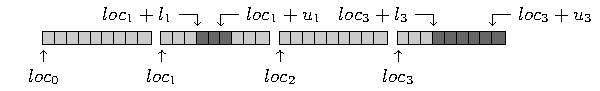
\includegraphics{img/lattice}
  \caption{The concrete semantics of $\gr(p)=\{\loc{1} + [3, 5],
    \loc{3} + [3, 8]\}$. Dark grey cells denote possible (concrete)
    values of $p$.}
  \label{fig:lattice}
\end{figure}

Now for the abstract operations: $(\bot,\ldots,\bot)$ is the least
element of our lattice, and $([-\infty,\infty],
\ldots,[-\infty,\infty])$ the greatest one. 

Given the two abstract values $\gr(p^1)=(p_0^1,\ldots p_{n-1}^1)$ 
and $\gr(p^2) =(p_0^2,\ldots
p_{n-1}^2)$, the union $\gr(p^1)\sqcup \gr(p^2)$ is the tuple
$(q_{0}, \ldots, q_{n-1})$ where: $$q_{i}
= \begin{cases} \begin{array}{cl} \perp & \mbox{ if } p_i^{1} = p_i^2=\mbox{ $\perp$ }  \\
  p_1\sqcup p_2 & \mbox{ else } \end{array} \end{cases}$$
and $\gr(p^1)\sqsubseteq \gr(p^2)$ if an only if all involved
(symbolic) intervals of $p^1$ are included in the ones of $p^2$: $\forall i \in [0..(n-1)], p_i^{1} \sqsubseteq p_i^2$ (considering $\bot \sqsubseteq R$ and $\bot \sqcup R=R$ for all
non-empty intervals R).
We call this structure, formed by $(\ranboxes \cupdot \bot)^n$ plus its
partial ordering the lattice $\memboxes$.

\begin{example}[label=normalization2]
\label{ex:normalization2}
For the example depicted in Figure~\ref{fig:ex3} where we only have two
malloc sites denoted by $\loc{0}$ and $\loc{1}$, we will obtain the
following results:
$\gr(p) = \gr(b) = \{\loc{0} + [0, 0]\}$,
$\gr(m_0) = \gr(s) = \{\loc{1} + [0, 0]\}$,
$\gr(e) = \loc{0} + [N, N]$,
$\gr(m_1) = \loc{1} + [1, +\infty]$,
$\gr(i_7) = \loc{0} + [N+strlen(m_0), N+strlen(m_0)+1]$.
How this mapping is found is discussed in the rest of this section.
\end{example}

\paragraph{Abstract semantics for \gr, and concretisation.}
The abstract semantics of each instruction in our core language is given by
Figure~\ref{fig:absSemanticsGR}.
Figure~\ref{fig:absSemanticsGR} defines a system of equations whose fixed
point gives us an approximation on the locations that each pointer may
dereference.
We remind the reader of our notation: $\lb{[l, u]} = l$, and
$\ub{[l, u]} = u$.
In Figure~\ref{fig:absSemanticsGR}, this notation surfaces in the semantics of
intersections.
The abstract interpretation of the pointer-related instructions in
Figure~\ref{fig:ex3} yields the results discussed in
Example~\ref{ex:normalization2}.

%\renewcommand{\arraystretch}{0.9}
\begin{figure}[htb!]
\begin{footnotesize}
$$\begin{array}{rcl}
\begin{aligned} j:p = \mbox{ malloc }(v) \\ \mbox{ with } v \mbox{
    scalar }\end{aligned} & \Rightarrow & 
\gr(p) = (\perp, \ldots, \underbrace{[0, 0]}_{j^{th} component}, \ldots)\\ \\
\begin{aligned} p = \mbox{ free }(v) \\ \mbox{ with } v \mbox{ scalar }\end{aligned} & \Rightarrow & 
\gr(p) = (\perp, \ldots, \mbox{ $\perp$ })\\ \\
\begin{aligned} v = v_{1} \end{aligned}& \Rightarrow &
\gr(v) = \gr(v_{1}) \\ \\
\begin{aligned} q = p + c \\ \mbox{ with } c \mbox{ scalar variable}%  \\ \mbox{ and
  % } \gr(p)=(p_0,\ldots p_{n-1}) 
\end{aligned}  & \Rightarrow &
\begin{cases} \gr(q) = (q_{0}, \ldots , q_{n-1}) \mbox{ with } \\ q_{i} = \begin{cases} 
\perp \mbox{if } p_{i} = \mbox{ $\perp$ } \\
p_i + R(c) \mbox{ else } \end{cases} \\ \end{cases} \\ \\
 q = \phi (p^1, p^2) & \Rightarrow &  \gr(q) = \gr(p^1)\sqcup
 \gr(p^2)\\ \\
q = p^1 \cap [-\infty, p^2] & \Rightarrow &
\begin{cases} 
\gr(q) = (q_{0}, \ldots, q_{n-1}) \mbox{ with } \\ q_{i}
= \begin{cases} \mbox{ $\perp$ } \mbox{ if (} p_i^1 = \mbox{ $\perp$ or } p_i^2 = \perp )\\
  p_i^1 \sqcap [-\infty, \ub{p_i^2}] \mbox{ else } \end{cases}\\
\end{cases} \\ \\
q = p^1 \cap [p^2, +\infty] & \Rightarrow &
\begin{cases} 
\gr(q) = (q_{0}, \ldots, q_{n-1}) \mbox{ with } \\ q_{i}
= \begin{cases} \mbox{ $\perp$ if (} p_i^1 = \mbox{ $\perp$ or } p_i^2 = \mbox{ $\perp$ } )\\
  p_i^1 \sqcap [\lb{p_i^2}, +\infty] \mbox{ else } \end{cases}\\
\end{cases}\\ \\
\begin{aligned} q = *p \end{aligned}& \Rightarrow &
\gr(q) = ([-\infty, \infty], \ldots, [-\infty, \infty]) \\ \\
\begin{aligned} *q = p \end{aligned}& \Rightarrow &
\mbox{\textsf{Nothing}} 
\end{array}$$
\caption{\label{fig:absSemanticsGR}Constraint generation for $\gr$
  with $\gr(p) = (p_0, \ldots, p_{n - 1})$ given $p$ in the right hand
  side of rules}
\end{footnotesize}
\end{figure}

There remains to define how the abstract states will be concretised
($@(\loc{i})$ is the actual address returned by the $i^{th}$ malloc):
%We define the concretisation function for a given abstract value as follows:
\begin{definition}[Concretisation]
\label{def:concretisation}
Given $\gr({p})$ an abstract value (a set of ``abstract addresses for
p''), denoted by $\gr(p)=(p_0,\ldots,p_{n-1})$ then we define its
concretisation as follows:
$$\gamma(\gr(p)) = \bigcup_{i \in \supp_{GR}(p)} \{@(\loc{i}) +
o, o \in p_i\}$$
\end{definition}
The concretisation function of this abstract value is thus a set of
(concrete) addresses, obtained by shifting a set of base addresses by a certain
value in \ranboxes\footnote{While speaking about symbolic ranges, we
  also have to concretize the values involved in the bounds of
  $p_i$, that is we shall use the actual values between $S(p_{i\downarrow})$
  and $S(p_{i\uparrow})$.}.

\begin{proposition}
  $(\alpha,\gamma)$ is a Galois connection.
\end{proposition}
\begin{proof}
  Immediate since $(\alpha_{\mbox{\ranboxes}},\gamma_{\mbox{\ranboxes}})$ is a
  galois connection.
\end{proof}
\paragraph{Solving the abstract system of contraints}

Following the abstract interpretation framework, we solve our
system of constraints by computing for each pointer a growing set of
abstract values until convergence.

However, as the underlying lattice $\ranboxes$ has infinite height,
widening is necessary to ensure that these sequence of iterations
actually terminate.  Our widening operation on pointers generalizes
the widening operation on ranges. It is defined as follows:

\begin{definition}
  Given $\gr(p)$ and $\gr(p')$ with $\gr(p) \sqsubseteq \gr(p')$, we
  define the widening operator:
  $$\gr(p)\nabla \gr(p')=(p_0\nabla p'_0, \ldots,p_{n-1}\nabla
  p'_{n-1}),$$
where $\nabla$ denotes the widening on \ranboxes, extended with $\bot
\nabla \bot =\bot$ and $\bot \nabla [l,u]=[l,u]$.
\end{definition}

As usual, we only apply the widening operator on a cut set of the
control flow graphs (here, only on $\phi$ functions). 

Widening may lead
our interpreter to produce very imprecise results. To recover part of
this imprecision, we use a descending sequence of finite size: after
convergence, we redo a step of symbolic evaluation of the program,
starting from the value obtained after convergence.
One example of analysis will be detailed later, in
Section~\ref{sub:wrap}.


\paragraph{The abstract interpretation of loads and stores.}
In Figure~\ref{fig:absSemanticsGR}, we chose not to
track precisely the intervals associated with pointers stored in
memory.
In other words, when interpreting stores, e.g., $q = *p$,
we assign the top value of our lattice to $q$.
This decision is pragmatic.
As we shall explain in Section~\ref{sec:exp}, a typical compilation
infra-structure already contains analyses that are able to track the propagation
of pointer information throughout memory.
Our goal is not to solve this problem.
We want to deliver a fast analysis that is precise enough to handle C-style
pointer arithmetic.

\subsection{Answering \gr Queries}
\label{sub:queriesGR}

Our queries are based on the following result, that is an immediate
consequence of the fact our analysis is an abstract interpretation:
 \begin{proposition}[Correctness]
Let $p$ and $p'$ be two pointers in a given program  then~:
$$ 
\begin{array}{cc}
\mbox{if }& \supp_{GR}(p) \cap \supp_{GR}(p') = \emptyset \\    
or& \forall i \in
\supp_{GR}(p) \cap \supp_{GR}(p'), p_i \sqcap p'_i = \emptyset
\end{array}$$
then $\gamma(\gr(p)) \cap \gamma(\gr(p')) = \emptyset$.

\end{proposition}
In other words, if the abstract values of two different pointers of
the program have a null intersection, then the two \emph{concrete
  pointers} do not alias. This result is directly implied by the
abstract interpretation framework.
Thanks to this result, we implement the query $Q_{\gr}(p,p')$ as~:
\begin{compactitem}
\item If $\gr(p)$ and $\gr(p')$ have an empty intersection, then
``they do not alias''.
\item Else  ``they may alias''.
\end{compactitem}

\subsection{Local Range Analysis of Pointers}
\label{sub:local}

The global pointer analysis is not path sensitive.
As a consequence, this analysis cannot, for instance, distinguish the effects
of different iterations of a loop upon the actual value of a pointer, or the
effects of different branches of a conditional test on that very pointer.
The program in Figure~\ref{fig:path_sensitiveness} illustrates this issue.
Pointers $a_4$ and $a_5$ clearly must not alias.
Yet, their abstract states have non-empty intersections for \loc{1}.
Therefore, the query mechanism of Section~\ref{sub:queriesGR} would return a
``may-alias" result in this case.

\begin{figure}[t!]
  \centering
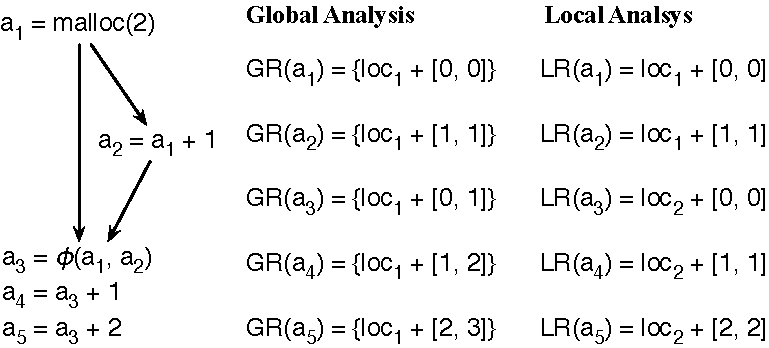
\includegraphics{img/path_sensitiveness}
  \caption{Example that illustrates imprecision of global analysis due to
  lack of path-sensitiveness.}
  \label{fig:path_sensitiveness}
\end{figure}

To solve this problem, we have developed a {\em local}
version of our pointer analysis.
We call it local because it creates new locations for every $\phi$-function.
Our local range analysis is simpler than its global counterpart.
We solve it in a single iteration of abstract interpretation applied on the
instructions of our core language.
Instructions are evaluated abstractly in the order given by
the program's dominance tree.
Figure~\ref{fig:absSemanticsLR} gives the abstract semantics of each
instruction.
The abstract value $\lr(p)$ exists in $({\mathcal L}oc\cup {\mathcal
  N}ewLocs)\times \ranboxes$ where ${\mathcal N}ewlocs$ denotes a set of
``fresh location variables'', that are computed by invocation of the
function ${\mathcal N}ewLocs()$. As before, we write $\loc{}+R$ instead of
$(\loc{}, R)$. Similarly to $\gamma_{GR}$, $\gamma_{LR}$ denotes the set
of abstract addresses from $@(\loc{})+R_{\downarrow}$ to
$@(\loc{})+R_{\uparrow}$.

\begin{figure}[t!]
\begin{footnotesize}
$$\begin{array}{rcl}
\begin{aligned} p = \mbox{ malloc }(v) \\ \mbox{ with } v \mbox{ scalar } \end{aligned} & \Rightarrow &
\lr(p) = {\mathcal N}ewLocs() + [0, 0]\\ \\
\begin{aligned} v = v_{1}\end{aligned}& \Rightarrow &
\lr(v) = \lr(v_{1})\\ \\
\begin{aligned} q = p + c \\ \mbox{ with } c \mbox{ scalar variable and} \\\lr(q) = \loc{i} + [l, u]\end{aligned}& \Rightarrow &
\lr(q) = \loc{i} + ([l, u] + R(c))\\ \\
j : q = \phi (p_{1},p_2) & \Rightarrow &
\lr(q) = {\mathcal N}ewLocs()  + [0, 0]\\ \\
\begin{aligned} q = p_1 \cap [-\infty, p_2] \\q = p_1 \cap [p_2, +\infty] \end{aligned} & \Rightarrow & \lr(q) = \lr(p_1)\\ \\
\begin{aligned} q = *p_{1} \end{aligned}& \Rightarrow &
\lr(q) = {\mathcal N}ewLocs() + [0, 0]\\ \\
\begin{aligned} *q = p_{1} \end{aligned}& \Rightarrow &
\mbox{\textsf{Nothing}} 
\end{array}$$
\caption{\label{fig:absSemanticsLR}Constraint generation for LR}
\end{footnotesize}
\end{figure}
To find a solution to the local analysis, we solve the system provided by the
abstract rules seen in Figure~\ref{fig:absSemanticsLR}.
This resolution process involves computing an increasing
sequence of abstract values for each pointer $p$ of the program.
Contrary to the global analysis, this analysis is based on a finite
lattice, we do not need any widening operator.
Figure~\ref{fig:path_sensitiveness} (Right) shows the result of the local
analysis.
Contrary to the global analysis, we have a new location bound to variable
$a_3$, which is defined by a $\phi$ operator.
The range of this new location is $[0, 0]$.
The other variables that are functions of $a_3$, e.g., $a_4$ and $a_5$, have
now non-intersection ranges associated with this new memory name.

\subsection{Answering \lr Queries}
\label{sub:queriesLR}

The correction for the local analysis is stated by the following proposition:
 \begin{proposition}[Correctness]
Let $p$ and $p'$ be two pointers in a given program, and $\gamma_{LR}$ be the
concretization of the abstract map $LR$, which we state like in
Definition~\ref{def:concretisation}.
If $\lr(p)=\loc{}+R$ and $\lr(p')=\loc{}'+R'$, then 
$\mbox{if }\loc{} = \loc{}' \mbox{ and }R\sqcap R'=\emptyset \mbox{ then
}\gamma(\lr(p))\cap \gamma(\lr(p')=\emptyset$.
In other words, $p$ and $p'$ never alias.
\end{proposition}
\medskip 
Thanks to this result, we implement the query $Q_{\lr}(p,p')$:
\begin{compactitem}
\item If $\lr(p)$ and $\lr(p')$ have a common base pointer with ranges
  that do not intersect, then ``they do not alias''.
\item Else  ``they may alias''.
\end{compactitem}

\subsection{Complexity}

The e-SSA representation ensures that we can implement our analysis sparsely.
Sparsity is possible because the e-SSA form renames variables at each program
point where new abstract information, e.g., ranges of integers and pointers,
arises.
According to Tavares {\em et al.}~\citep{Tavares14}, this property -- single
information -- is sufficient to enable sparse implementation of non-relational
static analyses~\citep{Tavares14}.
Therefore, the abstract state of each variable is invariant along the
entire live range of that variable.
Consequently, the space complexity of our static analysis is $O(|V|\times I)$,
where $V$ is the set of names of variables in the program in e-SSA form, and
$I$ is a measure of the size of the information that can be bound to each
variable.

We apply widening after one iteration of abstract interpretation.
Thus, we let the state of a variable to change first from $[\bot, \bot]$ to
$[s_l, s_u]$, where $s_l \neq -\infty$, and $s_u \neq +\infty$.
From there, we can reach either $[-\infty, s_u]$ or $[s_l, +\infty]$.
And, finally, this abstract state can jump to $[-\infty, +\infty]$.
Hence, our time complexity is $O(3 \times |V|) = O(|V|)$.
This observation also prevents our algorithm from generating expressions with
very long chains of ``min'' and ``max'' expressions.
Therefore, $I$, the amount of information associate with a variable, can be
represented with $O(1)$ space.
As a consequence of this frugality, our static analysis runs in $O(|V|)$ time,
and requires $O(|V|)$ space.

\subsection{A wrap-up Example}
\label{sub:wrap}

Example~\ref{ex:widening} shows how our analysis works on the
program seen in Figure~\ref{fig:exmotiv}.

\begin{example}[label=widening]
\label{ex:widening}
Figure~\ref{fig:ex3} shows the control flow graph (CFG) of the program
in Figure~\ref{fig:exmotiv}. Our graph is in e-SSA
form~\citep{Bodik00}. Figure~\ref{fig:exWidening} shows the result
of widening ranges after one round of abstract interpretation (stabilization 
achieved), and a descending sequence of size two.  Our system
stabilizes after each instruction is visited four times.  The first
visit does initialization, the second widening (and stabilization
check), and the last two build the descending sequence.
\end{example}

%\renewcommand{\arraystretch}{1.1}
\begin{figure}[t!]
\begin{footnotesize}
\centering
$$\begin{array}[c]{clcc}
\mbox{} & \mbox{Var} &           \gr & \lr  \\ \hline
& b, p, i_{0} & ([0, 0], \bot) & \loc{0} + [0, 0]\\
& m_{0}, s & (\bot, [0, 0]) & \loc{1} + [0, 0]\\ 
& i_{1} & ([0, 0], \bot) & \loc{2} + [0, 0]\\  
& i_{2} & ([0, 0], \bot) & \loc{2} + [0, 0]\\ 
& t_0 & ([1, 1], \bot) & \loc{2} + [1, 1]\\ 
& e & ([N, N], \bot) & \loc{0} + [N, N]\\ 
\mbox{Starting}& i_{3} & ([1, 1], \bot) & \loc{2} + [1, 1]\\ 
\mbox{state} & i_{4} & (\bot,\bot) & \loc{2} + [0, 0]\\ 
& f &  ([k, k], \bot)  & \loc{0} + [k, k]\\
& m_{1} &  (\bot, [0, 0])  & \loc{3} + [0, 0]\\
& m_{2} &  (\bot, [1, 1])  & \loc{3} + [1, 1]\\ 
& i_{5} & (\bot,\bot) & \loc{4} + [0, 0] \\
& i_{6} & (\bot,\bot) & \loc{4} + [0, 0]\\
& i_{7} & (\bot,\bot) & \loc{4} + [1, 1]\\
\hline
& i_{1} &  ([0, +\infty], \bot) &\\ 
& i_{2} &  ([0, +\infty], \bot) & \\ 
& t_0 &  ([1, +\infty], \bot) & \\
 \mbox{Growing} & i_{3} & ([1, +\infty], \bot) & \\ 
 \mbox{iterations} & i_{4} & ([N, +\infty], \bot) & \\ 
\mbox{+ widening}& m_{1} & (\bot, [0, +\infty]) & \\ 
& m_{2} & (\bot, [1, +\infty]) & \\ 
& i_{5} & ([N, +\infty], \bot) & \\ 
& i_{6} & ([N, k-1], \bot) & \\ 
& i_{7} & ([N+1, k], \bot) & \\ 
\hline
& i_{2} & ([0, N-1], \bot) & \\ 
& t_0 & ([1, N], \bot) & \\
\mbox{After one} & i_{3} & ([1, N], \bot) & \\ 
\mbox{descending} & m_{1} & (\bot, [0, +\infty]) & \\ 
\mbox{step}& m_{2} & (\bot, [1, +\infty]) & \\
\hline
& i_{1} & ([0, N], \bot) &\\ 
\mbox{After two} & i_{3} & ([1, N], \bot) & \\ 
\mbox{descending} & i_{4} & ([N, N], \bot) & \\
\mbox{steps}& i_{5} & ([N, k], \bot) & \\
& i_{6} & ([k-1, k], \bot) & \\
& i_{7} & ([k, k+1], \bot) & \\ 
\end{array}$$
\caption{Abstract interpretation of CFG seen in Figure~\ref{fig:ex3}
  (program in Figure~\ref{fig:exmotiv}). For $\gr$, we 
associate \loc{0} with the \texttt{malloc} at line 17 and \loc{1} with the
\texttt{malloc} at line 18 (of the program).
Only changes in $\gr$ and $\lr$ are rewritten after the growing and 
descending iterations. We let k = N+\texttt{strlen}(m$_0$).}
\label{fig:exWidening}
\end{footnotesize}
\end{figure}

This example illustrates the need of widening to ensure termination.
Our program has a cycle of dependencies between pointers $i_1$, $i_2$ and $i_3$.
If not for widening, pointer $i_3$, incremented in line 5 of
Figure~\ref{fig:exmotiv} would grow forever.
Thus, as in Abstract Interpretation, we must break
the cyclic dependences between our pointers under analysis, by means
of insertion of widening points (identify points in the CFG where to
apply widening to insure convergence).

Returning to our example of Figure~\ref{fig:exmotiv}, we are
interested in knowing, for instance, that the memory access at line 6 is 
independent on the accesses that happen at line 10.  To achieve
this goal, we must bound the memory regions covered by pointers $i_3$ and i$_7$.  A
cyclic dependence happens at the operation \texttt{i++}, because in this case,
we have a pointer being used as both, source and destination of the
update. Thus, we should have inserted a widening point at
stores and load instructions. 
However, in the Abstract Interpreter depicted in
Figure~\ref{fig:absSemanticsGR}, it was sufficient to insert widening
points at $\phi$ functions (as we already said before) because~:
\begin{compactitem}
\item heads of loops are $\phi$ functions (thus dependencies between
  variables of different iteration of loops are broken).
\item we are working on (e-)SSA form programs; thus, the only
  inter-loop dependencies are successive stores to the same variable~:
  \texttt{*q=..., *q=...}. The value $\gr(q)$
  is the union of all information gathered inside the loop. (In
  essence, memory addresses {\em are not} in static single assignment
  form, i.e., we could have the same address being used as the target
  of a store multiple times). This information might grow forever;
  hence, we would have inserted a widening point on the last write. In
  our case, the information we store is already the top of our
  lattice; hence, there is no need for widening.
\end{compactitem}

%Chapter 4: Experiments
\chapter{Experiments}
\label{chap:exp}

We have implemented our range analysis in the LLVM compiler, version 3.5.
In this section, we show a few numbers that we have obtained with this
implementation.
All our experiments have been performed on an Intel i7-4770K, with 8GB of
memory, running Ubuntu 14.04.2.
Our goal with these experiments is to show:
(i) that our alias analysis is more precise than other alternatives of
practical runtime; and
(ii) that it scales up to large programs.

\paragraph{On the Precision of our Analysis.}
In this section, we compare our analysis against the other pointer analyses
that are available in LLVM 3.5, namely {\em basic} and {\em SCEV}.
The first of them, although called ``basic", is currently the most effective
alias analysis in LLVM, and is the default choice at the -O3 optimization
level.
It relies on a number of heuristics to disambiguate
pointers\footnote{This list has been taken from the LLVM documentation,
available at \texttt{http://llvm.org/docs/AliasAnalysis.html} in September of
2015}:
\begin{compactitem}
\item Distinct globals, stack allocations, and heap allocations can never alias.
\item Globals, stack allocations, and heap allocations never alias the null
pointer.
\item Different fields of a structure do not alias.
\item Indexes into arrays with statically differing subscripts cannot alias.
\item Many common standard C library functions never access memory or only read
memory.
\item Function calls cannot reference stack allocations which never
escape from the function that allocates them
\end{compactitem}
As we see from the above list, the {\em basic} alias analysis has some of the
capabilities of the technique that we present in this work, namely the
ability to distinguish fields and indices within aggregate types.
In this case, such disambiguation is only possible when the aggregates
are indexed with constants known at compilation time.
For situations when these indices are symbols, LLVM relies on a second kind of
analysis to perform the disambiguation: the ``scalar-evolution-based" (SCEV)
alias analysis.
This analysis tries to infer closed-form expressions to the induction variables
used in loops.
For each loop such as:
\begin{verbatim}
for (i = B; i < N; i += S) { ... a[i] ... }
\end{verbatim}
this analysis associates variable \texttt{i} with the expression
$\mathtt{i} = \mathtt{B} + \mathit{iter} \times S, \mathtt{i} \leq \mathtt{N}$.
The parameter {\em iter} represents the current iteration of the loop.
With this information, SCEV can track the ranges of indices which
dereference array \texttt{a} within the loop.
Contrary to our analysis, SCEV is only effective to disambiguate pointers
accessed within loops and indexed by variables in the expected closed-form.

\begin{table}[t!]
\begin{center}
\begin{footnotesize}
{\renewcommand{\arraystretch}{1.1}
\begin{tabular}{|l|r|r|r|r|r|}
\hline
\textbf{{\footnotesize Program}} & \textbf{{\footnotesize \#Queries}} & \textbf{{\footnotesize \%scev}} & \textbf{{\footnotesize \%basic}}& \textbf{{\footnotesize \%rbaa}} & \textbf{{\footnotesize \%(r + b)}} \\ \hline
cfrac    & 89,255 & 0.87 & 9.70 & 16.65 & 21.03 \\
espresso &787,223&2.39&12.62&28.16    & 33.04 \\
gs       &608,374&15.56&40.67&56.18         & 59.99 \\
allroots &974&16.32&64.37&79.77      & 79.88 \\
archie   &159,051&0.98&20.57&16.44      & 28.04 \\
assembler&35,474&2.16&40.31&47.86    & 55.61 \\
bison    &114,025&0.74&10.95&9.56        & 14.74 \\
cdecl    &301,817&13.74&24.80&49.72      & 50.73 \\
compiler &9,515&0.49&67.27&67.27      & 69.20 \\
fixoutput&3,778&0.11&88.30&83.17     & 90.37 \\
football &495,119&3.58&59.20&60.08    & 65.08 \\
gnugo    &13,519&9.23&60.89&78.21        & 79.29 \\
loader   &13,782&2.32&29.55&36.47       & 46.09 \\
plot2fig &27,372&2.90&24.09&46.45     & 49.54 \\
simulator&25,591&3.56&46.32&41.25    & 52.27 \\
unix-smail&61,246&1.22&37.36&42.92   & 48.95 \\
unix-tbl &85,339&7.30&44.38&33.92     & 48.83 \\
anagram  &3,114&2.18&32.85&53.31       & 59.54 \\
bc       &198,674&14.14&30.95&47.86         & 50.01 \\
ft       &7,660&2.73&5.23&24.65             & 25.91 \\
ks       &14,377&0.61&22.98&21.60           & 27.70 \\
yacr2    &38,262&0.20&7.22&12.83         & 14.48 \\ \hline
Total    &3,093,541&6.97&30.83&41.73      & 46.53 \\ \hline
\end{tabular}}
\end{footnotesize}
\end{center}
\caption{Comparison between three different alias analyses.
We let \textbf{r + b} be the combination of our technique and the {\em basic}
alias analysis of LLVM.
Numbers in \textbf{scev}, \textbf{basic}, \textbf{rbaa} and \textbf{r+b}
show percentage of queries that answer ``no-alias".}
\label{fig:multisources}
\end{table}

Figure~\ref{fig:multisources} shows how the three different analyses fare
when applied on larger benchmarks.
For this experiment we have chosen three benchmarks that have been used in
previous work that compares pointer analyses:
Prolangs~\citep{Ryder01}, PtrDist~\citep{Zhao05} and MallocBench~\citep{Grunwald93}.
We first notice that in general all the pointer analyses in LLVM
disambiguate a relatively low number of pointers.
This happens because many pointers are passed as arguments of functions, and,
not knowing if these functions will be called from outside the program, the
analyses must, conservatively, assume that these parameters may alias.
Second, we notice that our pointer analysis is one order of magnitude more
precise than the scalar-evolution based implementation available in LLVM.
Finally, we notice that we are able to disambiguate more queries than the
{\em basic} analysis.
Furthermore, our results complements it in non-trivial ways.
In total, we tried to disambiguate 3.093 million pairs of pointers.
Our analysis found out that 1.29 million pairs reference non-overlapping
regions.
The {\em basic} analysis has been able to distinguish 953 thousand pairs.
By combining these two analyses, we extended this number to 1.439 thousand pairs
of pointers.
SCEV could not increase this number any further.

\begin{table}[b!]
\begin{center}
\begin{footnotesize}
{\renewcommand{\arraystretch}{1.1}
\begin{tabular}{|l|r|r|l|r|r|}
\hline
\textbf{{\footnotesize Prog}} & \textbf{{\footnotesize noalias}} & 
\textbf{{\footnotesize global}} & \textbf{{\footnotesize Prog}}& 
\textbf{{\footnotesize noalias}} & \textbf{{\footnotesize global}} \\ \hline
cfrac & 14,865 & 1,102 & gnugo & 10,573 & 1,851 \\
espresso & 221,416 & 20,791 & loader & 5,026 & 433 \\
gs & 341,532 & 106,859 & plot2fig & 12,713 & 861 \\
allroots & 777 & 182 & simulator & 10,557 & 1,092 \\
archie & 26,142 & 2,034 & unix-smail & 26,289 & 771 \\
assembler & 16,977 & 905 & unix-tbl & 28,948 & 1,136 \\
mybison & 10,905 & 1,417 & anagram & 1,660 & 88 \\
cdecl & 150,050 & 43,619 & bc & 95,091 & 32,498 \\
compiler & 6,401 & 156 & ft & 1,888 & 452 \\
fixoutput & 3,142 & 4 & ks & 3,105 & 218 \\
football & 297,491 & 22,052 & yacr2 & 4,909 & 487 \\ \hline
\end{tabular}}
\end{footnotesize}
\end{center}
\caption{Number of queries solved with the global test of
Section~\ref{sub:global}.
Column \textbf{noalias} gives the number of queries that we have been able
to disambiguate, and column \textbf{global} shows how many queries were solved
with the global test.}
\label{fig:noalias}
\end{table}

Figure~\ref{fig:noalias} shows the proportion of queries that we have been
able to disambiguate with the global test of Section~\ref{sub:global}.
The two columns \textbf{noalias} of Figure~\ref{fig:noalias} correspond to the
percentage in column \textbf{\%rbaa} applied on the column \textbf{\#Queries}
of Figure~\ref{fig:multisources}.
Overall, the global test has given us 239,008, out of 1,290,457 ``no-alias''
answers.
This corresponds to 18.52\% of all the pairs of pointers that we have
disambiguated.
We did not show the local test in this table because these two tests are
not directly comparable.
The global test disambiguate pointers, and the local test disambiguate
the addresses used in instructions such as loads and stores.
These instructions can use pointers that might dereference overlapping regions;
however, not at the same moment during the execution of
the program.
The local test has been able to disambiguate 6.55\% of all the addresses used
in our benchmarks.
The rest of the disambiguation was obtained by comparing off-sets from different
locations.

% Precision, runtime, complexity, space, effectiveness
\paragraph{On the Scalability of our Analysis.}
The chart in Figure~\ref{fig:TimeVsSize} shows how our analysis scales
when applied on programs of different sizes.
We have used the 50 largest programs in the LLVM benchmark suite.
These programs gave us a total of 800,720 instructions in the LLVM intermediate
representation, and a total of 241,658 different pointer variables.
We analyzed all these 50 programs in 8.36 seconds.
We can -- effectively -- analyze 100,000 instructions in about
one second.
In this case, we are counting only the time to map variables to values in
\ranboxes.
We do not count the time to query each pair of pointers, because usually
compiler optimizations perform these queries selectively, for instance, only
for pairs of pointers within a loop.
Also, we do not count the time to run the out-of-the-box implementation of
range analysis mentioned in Section~\ref{sub:sra}, because our version of it
is not implemented within LLVM.
It runs only once, and we query it afterwards, never having to re-execute it.

\begin{figure}[t!]
  \centering
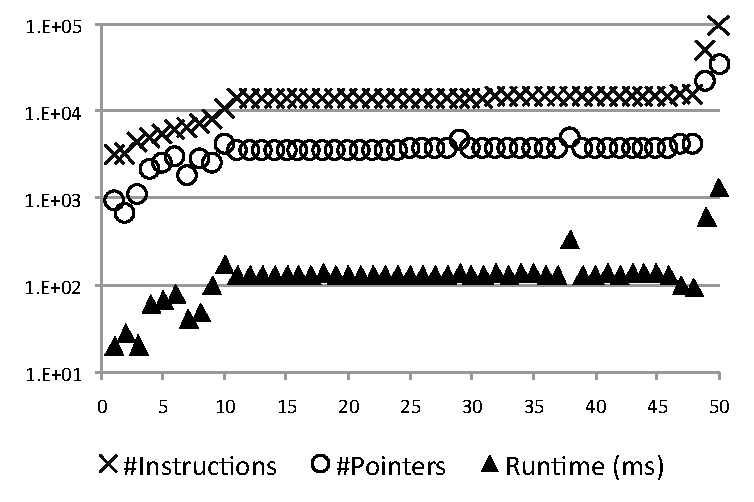
\includegraphics{img/TimeVsSize}
  \caption{Runtime of our analysis for the 50 largest benchmarks in the LLVM
  test suite. Each point on the X-axis represents a different benchmark.
  Benchmarks are ordered by size.
  This experiment took less than 10 seconds.}
  \label{fig:TimeVsSize}
\end{figure}

The chart in Figure~\ref{fig:TimeVsSize} provides strong visual indication of
the linear behavior of our algorithm.
We have found, indeed, cogent evidence pointing in this direction.
The linear correlation coefficient ($R$) indicates how strong is a linear
relationship between two variables.
The closer to one, the more linear is the correlation.
The linear correlation between time and number of instructions for the
programs seen in Figure~\ref{fig:TimeVsSize} is 0.982, and the
correlation between time and number of pointers is 0.975.

%Chapter 5: Final Thoughts
\chapter{Final Thoughts}
\label {chap:final}
\section {Limitations}
%- Limitations of the current analysis
Using the symbolic range analysis for comparing offsets is inherently 
imprecise. Issues lie on comparing two symbolic expressions and its 
difficulties, especially on comparing lower bounds with upper bounds from two
different variables, and on local relationships of variables with overlapping 
ranges.

Figure \ref{fig:lim1} shows the first issue. Analyzing this algorithm, the 
symbolic range analysis returns the following ranges: $R(\sigma_a) = [a, b-1]$,
$R(\sigma_b) = [a+1, b]$. This impedes the disambiguation of the two array 
accesses, $V[\sigma_a]$ and $V[\sigma_b]$, since it is impossible to prove that
 the ranges of $\sigma_a$ and $\sigma_b$ do not overlap. To do so, it would be 
 necessary for the valuation of symbolic expressions to be able to say that 
 $b-1 < a+1$ or that $b < a$, which it cannot do. So in this example, even 
 though it is obvious that the two array accesses cannot alias to the same 
 location, since their offsets are obligatorily different by the $if$ 
 condition. 
 
Figure \ref{fig:lim2} shows the second issue. It again shows two array accesses 
that are obviously disjoint that our analysis cannot disambiguate. Analyzing this 
algorithm, the symbolic range analysis returns the following ranges: 
$R(i) = [0, 9]$, $R(j) = [1, 10]$. It's clear that these ranges overlap and 
that our analysis could not say that they are disjoint even though, at the 
array accesses, $j$ is aways different and greater than $i$. 

These examples show two very interesting limitations of our analysis. They 
both can disable optimizations such as automatic parallelization of code and 
loop invariant code motion on some cases in which these optimizations might be 
desirable. It is clear that simply verifying if two offset ranges are disjoint 
is not enough to achieve ideal precision, since they can hide relationships 
between variables that are aways true when the two variables are alive and 
that can help in disambiguating two pointers, even if there is a relationship 
between these pointers or between the offsets that constitute such pointers. 
 

\begin{figure}[t!]
  \centering
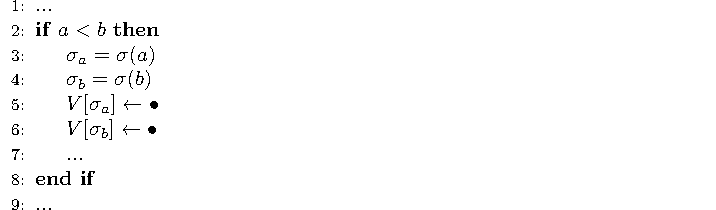
\includegraphics[width=\linewidth]{img/limitation}
  \caption{}
  \label{fig:lim1}
\end{figure}

\begin{figure}[t!]
  \centering
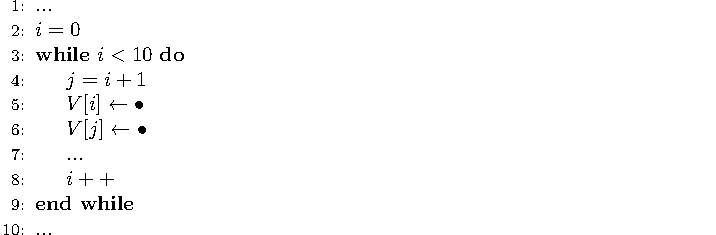
\includegraphics[width=\linewidth]{img/limitation2}
  \caption{}
  \label{fig:lim2}
\end{figure}

\section {Future Work}
The reason for the limitations exposed before lays on the fact that our analysis 
use range intervals to disambiguate pointers.
In the examples of figure \ref{fig:lim1} and figure \ref{fig:lim2}, the ranges 
of integer variables might either overlap or aren't comparable. But, in the 
examples, variables do have relationships between them that allow for 
disambiguation in the form of inequalities ($a<b$ and $i<j$). To take advantage 
of such relationships we intend to use a lattice similar to Pentagons.

Pentagons is an abstract domain invented by Logozzo and F\"{a}hndrich
to infer symbolic bounds to the integer variables used in
programs \citep{Logozzo08,Logozzo10}.
This abstract domain is formed by the combination of two
lattices.
The first lattice is the {\em integer interval domain} \citep{Cousot77}, which
maps integer variables to ranges $[l, u]$ of numeric lower ($l$) and upper ($u$)
bounds.
The second lattice is the {\em strict upper bound}, which maps each variable
$v$ to a set $L_<$ of other variables, so that if $u \in L_<(v)$, at a given
program point $\mathtt{p}$, then $u < v$ at $\mathtt{p}$. 

Since their debut \citep{Logozzo08}, Pentagons have been used in several
different ways.
For instance, Logozzo and F\"{a}hndrich have employed this domain to eliminate
array bound checks in strongly typed programming
languages \citep{Logozzo10}, and to ensure absence of division by zero or
integer overflows in programs.
Moreover, Nazar\'{e} {\em et al.} \citep{Nazare14} have used Pentagons to reduce
the overhead imposed by AddressSanitizer \citep{Serebryany12} to guard C against
out-of-bounds memory accesses.
The appeal of pentagons comes from two facts.
First, this abstract domain can be computed efficiently -- in quadratic time on
the number of program variables.
Second, as an enabler of compiler optimizations, Pentagons have been
proven to be substantially more effective than other forms of abstract
interpretation of similar runtime \citep{Logozzo08}.

%- Future Work
Our initial and recent use of pentagons for such purpose has been successful. 
It is able to handle programs as large as SPEC's gcc in a few minutes and go
through SPEC CPU 2006 \citep{Henning06} in able time. It has proven very 
useful in some cases, such as SPEC \texttt{470.lbm}.  
In further future work, we plan to investigate better splitting strategies
and other more expressive lattices to improve the global precision of
our analyses.

\section {Final Conclusions}
%- Final Conclusions
In this work we have presented a new alias analysis technique that handles,
within the same theoretical framework, the subtleties of pointer arithmetic
and memory indexation.
Our technique can disambiguate regions within arrays and C-like structs using
the same abstract interpreter.
We have achieved precision in our algorithm by combining
alias analysis with classic range analysis on the symbolic domain.
Our analysis is fast, and handles cases that the implementations of
pointer analyses currently available in LLVM cannot deal with.

Apart from this contribution, there is plenty to study on the area of 
pointer analysis, and the area of pointer arithmetics still needs quite a bit 
of research. Its dire need are very efficient static analyses that run fast on 
very big programs and very lean dynamic analyses and monitors. Our focus has 
been on the static analysis side. Lazy implementations, where main computations 
are made on the query moment, seem to be a very promising take on alias 
analyses and can expedite runtime. Focus on integrating new proposals to 
bigger compilation frameworks and existing optimizations should also be explored 
by the community on an effort of making new technology more usable across 
researchers and projects. There is still a lot of work to be done and we hope 
that our contribution can be only a building block of a much bigger effort from 
many more scientists.

% Aqui vem a parte da bibliografia: use o comando \ppgccbibliography indicando
% apenas o nome do arquivo .bib (sem a extens�o).
\ppgccbibliography{bibfile}





\end{document}
